\documentclass{standalone}
\usepackage{tikz}
\usetikzlibrary{patterns, positioning}

\begin{document}
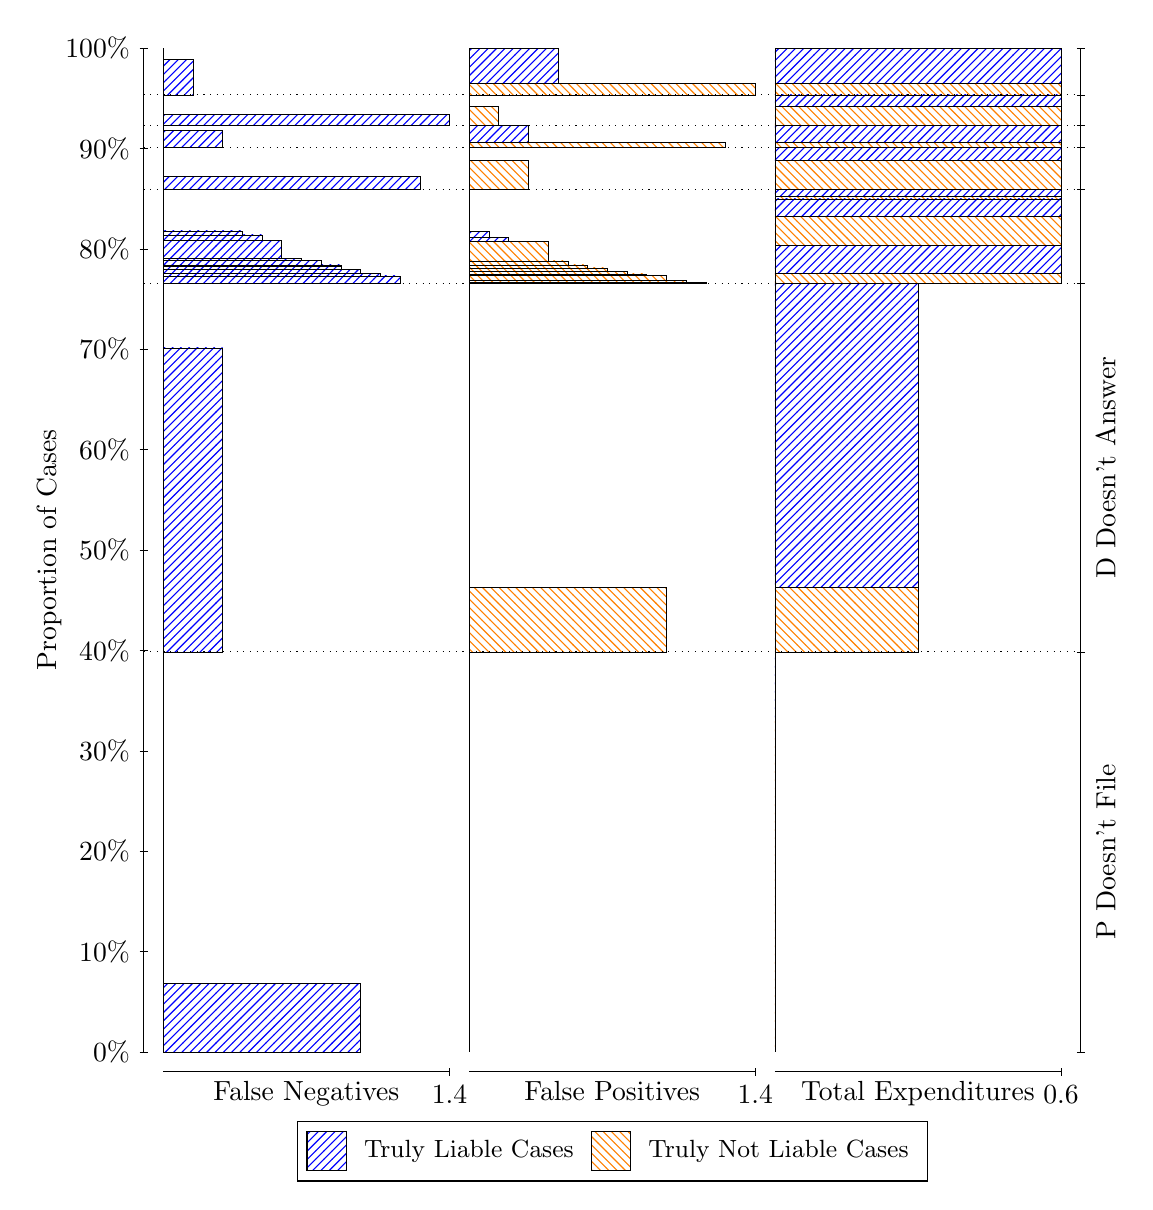
\begin{tikzpicture}
\draw[black, very thin] (1.5,1.75) -- (1.5,14.5);
\node[rotate=90, anchor=center] at (0.3, 8.125) {Proportion of Cases};
\draw[black, very thin] (1.45,1.75) -- (1.55,1.75);
\node[anchor=east] at (1.45, 1.75) {0\%};
\draw[black, very thin] (1.45,3.025) -- (1.55,3.025);
\node[anchor=east] at (1.45, 3.025) {10\%};
\draw[black, very thin] (1.45,4.3) -- (1.55,4.3);
\node[anchor=east] at (1.45, 4.3) {20\%};
\draw[black, very thin] (1.45,5.575) -- (1.55,5.575);
\node[anchor=east] at (1.45, 5.575) {30\%};
\draw[black, very thin] (1.45,6.85) -- (1.55,6.85);
\node[anchor=east] at (1.45, 6.85) {40\%};
\draw[black, very thin] (1.45,8.125) -- (1.55,8.125);
\node[anchor=east] at (1.45, 8.125) {50\%};
\draw[black, very thin] (1.45,9.4) -- (1.55,9.4);
\node[anchor=east] at (1.45, 9.4) {60\%};
\draw[black, very thin] (1.45,10.675) -- (1.55,10.675);
\node[anchor=east] at (1.45, 10.675) {70\%};
\draw[black, very thin] (1.45,11.95) -- (1.55,11.95);
\node[anchor=east] at (1.45, 11.95) {80\%};
\draw[black, very thin] (1.45,13.225) -- (1.55,13.225);
\node[anchor=east] at (1.45, 13.225) {90\%};
\draw[black, very thin] (1.45,14.5) -- (1.55,14.5);
\node[anchor=east] at (1.45, 14.5) {100\%};

\draw[black, very thin] (13.4,1.75) -- (13.4,14.5);
\draw[black, very thin] (13.35,1.75) -- (13.45,1.75);
\node[anchor=west] at (13.35, 1.75) {};
\draw[black, very thin] (13.35,6.8304) -- (13.45,6.8304);
\node[anchor=west] at (13.35, 6.8304) {};
\draw[black, very thin] (13.35,11.513) -- (13.45,11.513);
\node[anchor=west] at (13.35, 11.513) {};
\draw[black, very thin] (13.35,12.708) -- (13.45,12.708);
\node[anchor=west] at (13.35, 12.708) {};
\draw[black, very thin] (13.35,13.235) -- (13.45,13.235);
\node[anchor=west] at (13.35, 13.235) {};
\draw[black, very thin] (13.35,13.514) -- (13.45,13.514);
\node[anchor=west] at (13.35, 13.514) {};
\draw[black, very thin] (13.35,13.905) -- (13.45,13.905);
\node[anchor=west] at (13.35, 13.905) {};
\draw[black, very thin] (13.35,14.5) -- (13.45,14.5);
\node[anchor=west] at (13.35, 14.5) {};

\draw[black, very thin, pattern color=blue, pattern=north east lines] (1.75,1.75) rectangle (4.2557,2.6245);
\draw[black, very thin, pattern color=orange, pattern=north west lines] (1.75,2.6245) rectangle (1.75,6.8304);
\draw[black, very thin, pattern color=blue, pattern=north east lines] (1.75,6.8304) rectangle (2.5017,10.693);
\draw[black, very thin, pattern color=orange, pattern=north west lines] (1.75,10.693) rectangle (1.75,11.513);
\draw[black, very thin, pattern color=blue, pattern=north east lines] (1.75,11.513) rectangle (4.7569,11.607);
\draw[black, very thin, pattern color=blue, pattern=north east lines] (1.75,11.607) rectangle (4.5063,11.642);
\draw[black, very thin, pattern color=blue, pattern=north east lines] (1.75,11.642) rectangle (4.2557,11.686);
\draw[black, very thin, pattern color=blue, pattern=north east lines] (1.75,11.686) rectangle (4.0052,11.732);
\draw[black, very thin, pattern color=blue, pattern=north east lines] (1.75,11.732) rectangle (4.0052,11.747);
\draw[black, very thin, pattern color=blue, pattern=north east lines] (1.75,11.747) rectangle (3.7546,11.807);
\draw[black, very thin, pattern color=blue, pattern=north east lines] (1.75,11.807) rectangle (3.504,11.831);
\draw[black, very thin, pattern color=blue, pattern=north east lines] (1.75,11.831) rectangle (3.2534,12.053);
\draw[black, very thin, pattern color=blue, pattern=north east lines] (1.75,12.053) rectangle (3.0029,12.128);
\draw[black, very thin, pattern color=blue, pattern=north east lines] (1.75,12.128) rectangle (2.7523,12.179);
\draw[black, very thin, pattern color=orange, pattern=north west lines] (1.75,12.179) rectangle (1.75,12.708);
\draw[black, very thin, pattern color=blue, pattern=north east lines] (1.75,12.708) rectangle (5.0075,12.868);
\draw[black, very thin, pattern color=orange, pattern=north west lines] (1.75,12.868) rectangle (1.75,13.235);
\draw[black, very thin, pattern color=blue, pattern=north east lines] (1.75,13.235) rectangle (2.5017,13.453);
\draw[black, very thin, pattern color=orange, pattern=north west lines] (1.75,13.453) rectangle (1.75,13.514);
\draw[black, very thin, pattern color=blue, pattern=north east lines] (1.75,13.514) rectangle (5.3833,13.658);
\draw[black, very thin, pattern color=orange, pattern=north west lines] (1.75,13.658) rectangle (1.75,13.905);
\draw[black, very thin, pattern color=blue, pattern=north east lines] (1.75,13.905) rectangle (2.1259,14.355);
\draw[black, very thin, pattern color=orange, pattern=north west lines] (1.75,14.355) rectangle (1.75,14.5);
\draw[black, very thin, pattern color=orange, pattern=north west lines] (5.6333,1.75) rectangle (5.6333,5.9559);
\draw[black, very thin, pattern color=blue, pattern=north east lines] (5.6333,5.9559) rectangle (5.6333,6.8304);
\draw[black, very thin, pattern color=orange, pattern=north west lines] (5.6333,6.8304) rectangle (8.1391,7.6503);
\draw[black, very thin, pattern color=blue, pattern=north east lines] (5.6333,7.6503) rectangle (5.6333,11.513);
\draw[black, very thin, pattern color=orange, pattern=north west lines] (5.6333,11.513) rectangle (8.6402,11.525);
\draw[black, very thin, pattern color=orange, pattern=north west lines] (5.6333,11.525) rectangle (8.3897,11.546);
\draw[black, very thin, pattern color=orange, pattern=north west lines] (5.6333,11.546) rectangle (8.1391,11.617);
\draw[black, very thin, pattern color=orange, pattern=north west lines] (5.6333,11.617) rectangle (7.8885,11.631);
\draw[black, very thin, pattern color=orange, pattern=north west lines] (5.6333,11.631) rectangle (7.6379,11.666);
\draw[black, very thin, pattern color=orange, pattern=north west lines] (5.6333,11.666) rectangle (7.3874,11.708);
\draw[black, very thin, pattern color=orange, pattern=north west lines] (5.6333,11.708) rectangle (7.1368,11.747);
\draw[black, very thin, pattern color=orange, pattern=north west lines] (5.6333,11.747) rectangle (6.8862,11.796);
\draw[black, very thin, pattern color=orange, pattern=north west lines] (5.6333,11.796) rectangle (6.6356,12.042);
\draw[black, very thin, pattern color=blue, pattern=north east lines] (5.6333,12.042) rectangle (6.1345,12.093);
\draw[black, very thin, pattern color=blue, pattern=north east lines] (5.6333,12.093) rectangle (5.8839,12.167);
\draw[black, very thin, pattern color=blue, pattern=north east lines] (5.6333,12.167) rectangle (5.6333,12.708);
\draw[black, very thin, pattern color=orange, pattern=north west lines] (5.6333,12.708) rectangle (6.3851,13.075);
\draw[black, very thin, pattern color=blue, pattern=north east lines] (5.6333,13.075) rectangle (5.6333,13.235);
\draw[black, very thin, pattern color=orange, pattern=north west lines] (5.6333,13.235) rectangle (8.8908,13.297);
\draw[black, very thin, pattern color=blue, pattern=north east lines] (5.6333,13.297) rectangle (6.3851,13.514);
\draw[black, very thin, pattern color=orange, pattern=north west lines] (5.6333,13.514) rectangle (6.0092,13.761);
\draw[black, very thin, pattern color=blue, pattern=north east lines] (5.6333,13.761) rectangle (5.6333,13.905);
\draw[black, very thin, pattern color=orange, pattern=north west lines] (5.6333,13.905) rectangle (9.2667,14.05);
\draw[black, very thin, pattern color=blue, pattern=north east lines] (5.6333,14.05) rectangle (6.7609,14.5);
\draw[black, very thin, pattern color=orange, pattern=north west lines] (9.5167,1.75) rectangle (9.5167,5.9559);
\draw[black, very thin, pattern color=blue, pattern=north east lines] (9.5167,5.9559) rectangle (9.5167,6.8304);
\draw[black, very thin, pattern color=orange, pattern=north west lines] (9.5167,6.8304) rectangle (11.333,7.6503);
\draw[black, very thin, pattern color=blue, pattern=north east lines] (9.5167,7.6503) rectangle (11.333,11.513);
\draw[black, very thin, pattern color=orange, pattern=north west lines] (9.5167,11.513) rectangle (13.15,11.64);
\draw[black, very thin, pattern color=blue, pattern=north east lines] (9.5167,11.64) rectangle (13.15,11.995);
\draw[black, very thin, pattern color=orange, pattern=north west lines] (9.5167,11.995) rectangle (13.15,12.364);
\draw[black, very thin, pattern color=blue, pattern=north east lines] (9.5167,12.364) rectangle (13.15,12.583);
\draw[black, very thin, pattern color=orange, pattern=north west lines] (9.5167,12.583) rectangle (13.15,12.617);
\draw[black, very thin, pattern color=blue, pattern=north east lines] (9.5167,12.617) rectangle (13.15,12.708);
\draw[black, very thin, pattern color=orange, pattern=north west lines] (9.5167,12.708) rectangle (13.15,13.075);
\draw[black, very thin, pattern color=blue, pattern=north east lines] (9.5167,13.075) rectangle (13.15,13.235);
\draw[black, very thin, pattern color=orange, pattern=north west lines] (9.5167,13.235) rectangle (13.15,13.297);
\draw[black, very thin, pattern color=blue, pattern=north east lines] (9.5167,13.297) rectangle (13.15,13.514);
\draw[black, very thin, pattern color=orange, pattern=north west lines] (9.5167,13.514) rectangle (13.15,13.761);
\draw[black, very thin, pattern color=blue, pattern=north east lines] (9.5167,13.761) rectangle (13.15,13.905);
\draw[black, very thin, pattern color=orange, pattern=north west lines] (9.5167,13.905) rectangle (13.15,14.05);
\draw[black, very thin, pattern color=blue, pattern=north east lines] (9.5167,14.05) rectangle (13.15,14.5);
\draw[black, dotted] (1.5,6.8304) -- (13.4,6.8304);
\draw[black, dotted] (1.5,11.513) -- (13.4,11.513);
\draw[black, dotted] (1.5,12.708) -- (13.4,12.708);
\draw[black, dotted] (1.5,13.235) -- (13.4,13.235);
\draw[black, dotted] (1.5,13.514) -- (13.4,13.514);
\draw[black, dotted] (1.5,13.905) -- (13.4,13.905);
\draw[black, very thin] (1.75,1.5) -- (5.3833,1.5);
\node[anchor=north] at (3.5667, 1.5) {False Negatives};
\draw[black, very thin] (5.3833,1.45) -- (5.3833,1.55);
\node[anchor=north] at (5.3833, 1.45) {1.4};

\draw[black, very thin] (5.6333,1.5) -- (9.2667,1.5);
\node[anchor=north] at (7.45, 1.5) {False Positives};
\draw[black, very thin] (9.2667,1.45) -- (9.2667,1.55);
\node[anchor=north] at (9.2667, 1.45) {1.4};

\draw[black, very thin] (9.5167,1.5) -- (13.15,1.5);
\node[anchor=north] at (11.333, 1.5) {Total Expenditures};
\draw[black, very thin] (13.15,1.45) -- (13.15,1.55);
\node[anchor=north] at (13.15, 1.45) {0.6};

\node[black, centered, rotate=90] at (13.72, 4.2902) {P Doesn't File};
\node[black, centered, rotate=90] at (13.72, 9.1715) {D Doesn't Answer};






\draw (7.449999999999999,1.5) node[draw=none] (baseCoordinate) {};
\begin{scope}[align=center]
        \matrix[scale=0.5, draw=black, below=0.5cm of baseCoordinate, nodes={draw}, column sep=0.1cm]{
            \node[rectangle, draw, minimum width=0.5cm, minimum height=0.5cm, pattern=north east lines, pattern color=blue] {}; &
            \node[draw=none, font=\small] (B) {Truly Liable Cases}; &
            \node[rectangle, draw, minimum width=0.5cm, minimum height=0.5cm, pattern=north west lines, pattern color=orange] {}; &
            \node[draw=none, font=\small] (B) {Truly Not Liable Cases}; \\
            };
\end{scope}

\end{tikzpicture}
\end{document}